\chapter{绪论}
\section{研究背景和意义}
近年来,大语言模型(Large Language Models,LLMs)在各个领域的成功应用,已然成为推动人工智能发展的重要趋势。以OpenAI的GPT(Generative Pre-trained Transformer)系列为代表的大模型,不仅在自然语言处理(Natural Language Processing,NLP)领域表现卓越,更逐步被应用于金融、医疗、教育、科学研究等众多行业,成为赋能各行各业的核心技术。

大模型的优点在于其强大的生成能力和通用性,但也存在显著的缺点,比如高昂的计算成本、巨大的内存需求以及推理过程中的性能瓶颈。因此,在“大模型时代”,如何优化大模型的推理效率,降低资源消耗,已成为科研界和工业界亟待解决的核心问题。

当前主流的大模型(如GPT系列、Llama等)均为Decoder-Only架构,即只使用Transformer模型\cite{Transformer}中的解码器(Decoder)做生成\cite{GPT-1,Llama2}。Decoder采用自回归生成方式完成文本生成任务,其推理生成过程主要分为两个阶段:1) 预填充阶段(Prefilling),该阶段会将提示词(Prompt)中所有词元(token)嵌入为词向量并输入Decoder,主要执行通用矩阵矩阵乘(Generalized Matrix Multiplication,GEMM)运算2)解码阶段(Decoding),该阶段会逐token地计算和生成,主要执行通用矩阵向量乘(Generalized Matrix Vector Multiplication,GEMV)运算。

在“GPT式”大模型的整个推理过程中,解码阶段占据主导地位\cite{InferLinear},有数据表明,其代表性算子GEMV平均占据82.3\%的GPU运行时间,而预填充阶段的代表性算子GEMM的平均耗时只占2\%,剩下的一些非线性算子总占比不到20\%\cite{SamsungHotChips}。这使得GEMV算子成为大模型推理的主要性能瓶颈,针对GEMV的优化对于提升大模型的推理效率至关重要,具有重大研究价值。

与GEMM不同,GEMV的计算过程数据重用性低,矩阵的计算近乎流式,存在大量数据搬移操作,计算访存比低。这些特点决定了其为内存瓶颈任务,使得常用的计算密集型硬件如GPU的利用率低,难以充分发挥其硬件优势。虽然有技术将多个推理请求组成一个批次(batch),进而将将GEMV操作合并成为GEMM操作以提高数据利用率\cite{Orca},但是在边端场景下,用户数量十分有限,batch大小绝大多数情况为1,这时GEMV往往称为系统瓶颈\cite{CellularLogicInMemory}。

存内计算(Processing-in-Memory,PIM)是一种新兴的计算范式,其秉持将计算置于数据侧的以数据为中心的思想,旨在通过将计算单元集成至存储部件附近,以较高的传输带宽存取数据进行计算。采用此种架构的硬件往往能凭借其独有高速传输通道和简单存储结构的具备高存储高带宽和低能耗的优势,能够充分解决传统冯诺依曼计算架构中的内存瓶颈问题。

近些年来许多PIM硬件被设计和提出\cite{SamsungHBMPIM,AxDIMM,AiM,AlibabaPIM,UPMEMHotChips},在这其中UPMEM是目前较为成熟的商用存算一体硬件,其硬件特点包括:1)高带宽和高存储,聚合带宽能达到TB级别。2)高并行性,拥有2560个DPU,每个DPU 16个线程可以并发控制,能够以极细的粒度分割任务。3)高能效,存算一体架构减少了数据搬运的能耗开销。同时UPMEM也存在一些局限性:1)较弱的计算能力,对于浮点和乘除法缺乏硬件支持。2)通信开销大,与主机或DPU之间通信开销大。

UPMEM的优势使得其特别适合卸载GEMV算子进行加速:高带宽和高存储可以有效解决GEMV算子乃至大模型推理过程中的内存瓶颈问题,同时GEMV中的矩阵和向量可以任意粒度切分且无数据依赖可以充分并行。但是UPMEM较弱的计算能力使得在加速GEMV时不得不做一些设计避免性能劣化。如何从软件角度适配硬件加速,以及如何修改设计硬件优化其应用性能的软硬协同优化方案成为待深入研究的课题。

\section{国内外研究现状}
大模型由最初的Transformer\cite{Transformer}发展而来,经过几次的参数膨胀\cite{GPT-1,GPT-2,GPT-3}量变引起质变具有了非常强的通用智能,广泛应用于智能客服、文本生成、金融、电商、教育和医疗等等众多领域\cite{EdgeLLM}。参数膨胀引起了大模型的部署推理成本极大增高,边端用户难以本地推理即使是参数量最小的模型(7B)。这个时候许多大模型推理加速方法应运而生\cite{LLMInferSurveyTsingHua},其中模型量化能够有效地缓解大模型推理的内存瓶颈\cite{ModelQuant}。模型量化按照量化是时机可以分为量化感知训练、量化感知微调和训练后量化。按照量化的数制映射方式可以分为线性量化和非线性量化,其中以训练后线性量化的方式成本最为低廉和简单,这之中又许多出名的工作,LLM.int8\cite{LLMINT8}通过矩阵离群值分解以较低的精度损失做到了8bit权重8bit激活量化(W8A8量化)。SmoothQuant\cite{SmoothQuant}引入一种数学上的等价变换平滑了W8A8的激活量化和权重量化的难度。AWQ\cite{AWQ}作为一种仅权重量化,同样基于激活值分布对权重矩阵做分解实现了W4的量化。GPTQ\cite{GPTQ}通过机器学习的方式逐层量化大模型,使用少量数据集校准,能够将权重量化到惊人的3-4bit。ZeroQuant系列\cite{ZeroQuant1,ZeroQuant2,ZeroQuantFP}工作引入了多种推理加速手段包括知识蒸馏、低秩补偿来缓解W8A8甚至W8A4的量化带来的误差,并提出浮点数量化优化定点数量化的观点。

另一个能够显著加速大模型推理速度的方式是提升其推理过程中基本算子GEMV的性能\cite{InferLinear}。GEMV相比GEMM计算偏流式,计算强度和数据重用性都没那么高,诸如Strassen算法\cite{Strassen}等算法层面的优化在现代计算机系统上的实现并不一定高效。有效的GEMV优化都是在计算机系统层面,结合计算硬件合理布局数据减少访存的优化\cite{GPUGEMV},常见的方法包括分块、数据打包、寄存器优化等等。

近存计算能够有效缓解内存瓶颈的应用。早在上世纪七十年代左右,存内计算悄然萌芽\cite{CellularLogicInMemory,LogicInMemory}。上世纪九十年代,Wulf等人系统性地定义了内存墙(Memory Wall)\cite{MemoryWall},说明了CPU和内存速度不匹配的问题。有部分学者提出存内计算(PIM,Processing in Memory),希望在存储测引入计算减少数据的搬移以缓解内存墙的问题。RowClone\cite{RowClone}工作通过在DRAM的bank内同时打开多行并利用共享的行缓存器(row buffer)实现行之间的快速复制。Seshadri等人\cite{BitAndOr,Ambit}提出一系列工作,通过简单修改内存单元的电路实现快速批量的逻辑计算。

在本世纪10年代,3D堆叠架构技术的突破使得近存计算技术再度火热。与此同时由于AI大火,有许多专用于神经网络的PIM芯片被推出。三星的HBM-PIM\cite{SamsungHBMPIM},为HBM(High Bandwidth Memroy)的每个内存bank配备了专门用于16位浮点数乘加操作的PIM单元以处理神经网络中的矩阵操作。三星的另一个产品AxDIMM\cite{AxDIMM}其将DRAM芯片和FPGA处理单元集成到一块有着DDR4标准接口的主板上,用于加速向量嵌入查找(embedding lookup)。海力士的AiM\cite{AiM}基于GDDR6内存,同样每个bank集成PIM单元用于神经网络的计算。国内的阿里也推出过近存计算产品\cite{AlibabaPIM}用于加速AI任务。

近几年,UPMEM作为以第一款可以商用的近存计算处理器产品\cite{UPMEMHotChips},大受研究者青睐,其本身是一条有着标准DDR4接口的内存插块(Dual In-line Memory Module,DIMM),可以像正常的内存条一样插在Intel服务器上(一个服务器最多可以插入20条UPMEM)。每个UPMEM插块包含两个rank,每个rank有64个内存处理单元(Dram Processing Unit,DPU)。每个DPU都拥有一个14级流水的RISC处理器,拥有16个线程。同时每个DPU拥有二级存储结构,包括64KB的SRAM(称为WRAM)和64MB的DRAM(称为MRAM)。

UPMEM自出现以来有许多研究者以此硬件结合相关应用做出了许多工作,涉及、数据库\cite{Skyline,PIM-Model,PIM-Tree,PIM-Trie,PIM-DB,PIM-Scan,PIM—QueryCompile,PIM-Join}、生物基因\cite{DNAMapping,VariantCalling,RNA-seq,UpPipe,GAPiM}以及人工智能\cite{UPMEMEmbeddingLookups,UPMEMTraditionalML,UPMEMCNN,UPMEMGNN,PIM-DL,SwiftRL,PIM-Opt}等各个领域。其中,UPMEM的高并行和通信效率低的特性使得其非常适合用于加速神经网络的推理。Niloofar Zarif将UPMEM用于embedding lookup任务的卸载\cite{UPMEMEmbeddingLookups},对于目前较大的嵌入表(embedding table)加速效果尤为明显。Juan Gómez-Luna等人\cite{UPMEMTraditionalML}以简单直接的方式卸载了传统机器学习中的基础模型到UPMEM上,包括线性回归、逻辑回归、决策树、K均值聚类,并做了全面丰富的测试,但是测试结果无一表明这些模型的推理都遭受了严重的计算性能瓶颈。Prangon Das\cite{UPMEMCNN}等人在UPMEM上分别卸载了嵌入二值神经网络(Embedded Binary Neural Network ,eBNN)和YOLOv3(主要是卸载CNN的卷积操作),其主要思想是将卷积神经网络(CNNs)的权重量化到低bit位,再通过查找表(Look Up Table,LUT)查询低bit浮点数乘积,以消除浮点乘法运算,但这会严重降低模型的精度。最与本课题应用 场景相近的工作PIM-DL\cite{PIM-DL}使用UPMEM推理Bert,其通过将矩阵乘法转换为最近邻查找和向量加法,减少了对乘法的需求,从而提高了计算效率。但其最近邻查找是在CPU上完成的,而UPMEM只执行向量加法操作,并没将计算重担完全卸载到UPMEM上。

\section{研究内容和创新点}
结合研究背景和国内外研究现状不难看出,使用UPMEM推理神经网络的主要难点在于其羸弱的计算能力往往拖累系统整体性能,无法充分发挥PIM架构的高带宽优势,如何简化和避免复杂的计算是本研究课题的主要挑战。本课题主要的研究内容如图\ref{Content}所示,主要分为理论基础、实践优化和结果总结三个部分。理论基础部分主要围绕大模型推理加速和近存计算两大主题梳理基本概念,查阅相关文献,对研究现状进行分析,概括出GEMV的软件特点和UPMEM近存硬件的特性,为后续工作打下理论基础。实践优化部分由软硬件协同优化组成。软件层面在商用近存计算硬件UPMEM上设计相关算法并优化,硬件方面基于近存计算模拟器,针对软件层面的优化瓶颈修改硬件以提升性能。结果总结部分主要是设计实验对上面做出的优化算法进行测试并分析。我们将从四个维度和三个硬件平台上(CPU,GPU,UPMEM)设计实验并分析,包括1)矩阵向量乘算子的总吞吐;2)矩阵向量乘算子的能效比;3)算子执行时间的瓶颈进行分析;4)扩展性实验,分别测试算法的多线程扩展性和矩阵尺寸扩展性。基于上面的实验分析结果,总结优化效果,说明本次研究的不足并对未来进行展望。

\begin{figure}[!htbp]
	\centering
    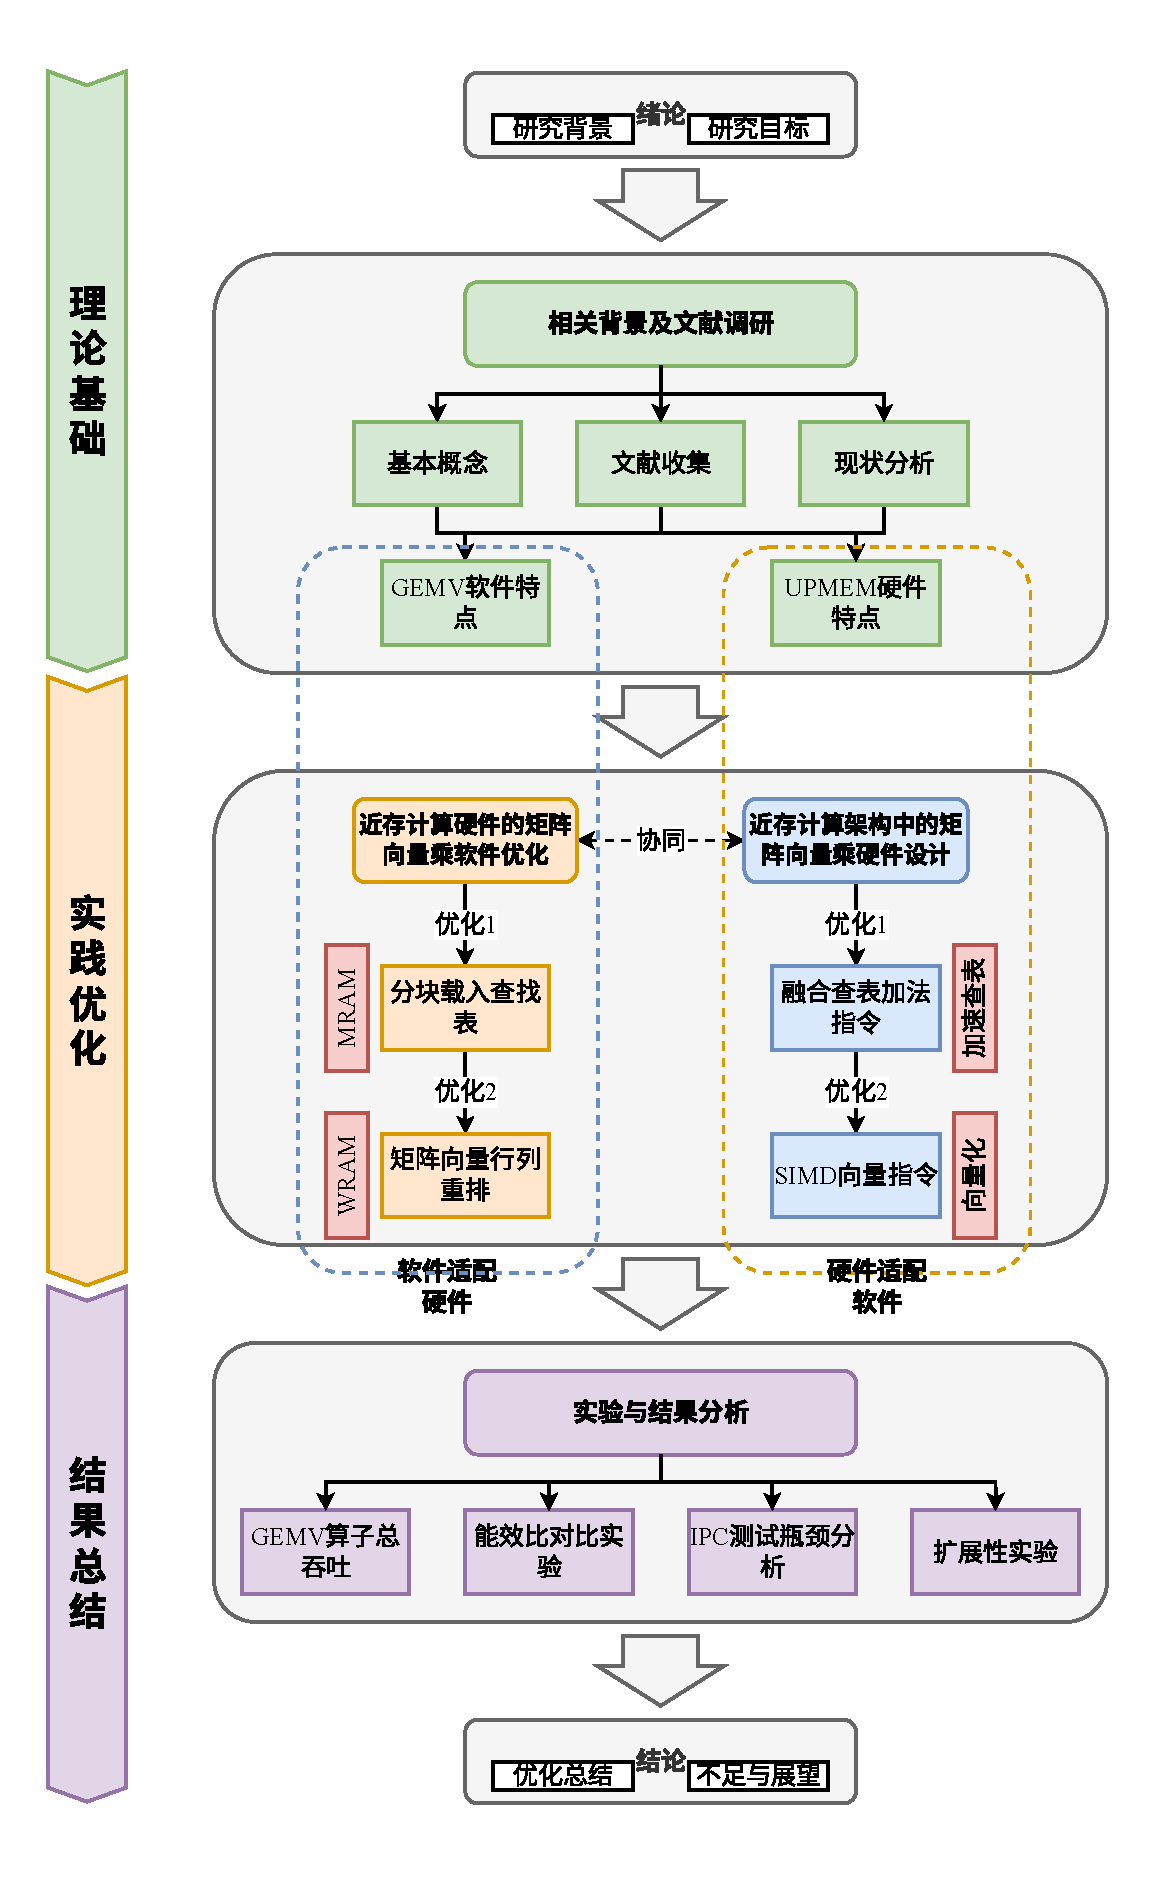
\includegraphics[width=0.9\textwidth]{figures/Content.pdf}
    \caption{研究内容路线图}
	\label{Content}
\end{figure}

基于上面的研究内容,概括本文的主要创新点如下:
\begin{itemize}
	\item [1)]
	通过文献阅读充分了解了UPMEM硬件的特点,设计基于查找表的矩阵向量乘算法,分别对两级存储结构(WRAM、MRAM)做出了优化:提出了针对数据主存(MRAM)访存优化的查找表分块算法LUT-M,通过分块载入查找表到工作缓存(WRAM)减少DMA访问数据主存(MRAM)主存次数增强的数据局部性;分别提出了针对工作缓存(WRAM)访存优化的矩阵行列重排算法,行重排算法LUT-W-R对矩阵的行进行重排减少GEMV中结果向量的读写次数从而减少对WRAM的访存。列重排算法LUT-W-C对矩阵进行列重排减少矩阵每一行计算中对查找表的访问从而减少WRAM的访问。这两种算法都减少数据从寄存器流出,增强寄存器的数据局部性,提升了GEMV算子的性能。
	\item [2)]
	通过分析基于查找表的矩阵向量乘算法的性能瓶颈,基于UPMEM的周期精确模拟器PIMulator修改增强UPMEM硬件:设计硬件单元增加了对融合查表加法指令的支持,主要用于优化UPMEM在进行查表时复杂的内存地址计算并融合加法到单条指令中,减少上述算法在每次做查表加法运算时的指令数目;设计增加向量单元以支持部分向量指令,包括向量加法、移位和重排,设计基于向量指令的查表矩阵向量乘算法LUT-SIMD,通过向量重排指令实现向量化查表,大大提升硬件计算能力和访存粒度,提升算法吞吐。
    \item [3)]
	对前两点的软硬协同优化设计了详细的基本测试,在CPU和GPU以及UPMEM三个硬件平台上,从四个维度进行实验,包括:测试各种优化算法下GEMV算子的总吞吐分析算子的绝对性能;测试三个平台下算子的能效比;测试各个算法优化下的执行时间的CPU和内存带宽利用率分析目前算子的性能瓶颈;最后进行扩展性测试,包括多线程扩展性测试和矩阵尺寸测试分析UPMEM应对不同尺寸矩阵的通用性。
\end{itemize}

\section{论文组织结构}
本文共六个章节组成,其中每个章节的主要内容如下:

第1章是全文的绪论。主要介绍了本文研究背景与意义、国内外研究现状、研究内容与创新点,并在最后介绍了全文的组织结构。

第2章是相关工作。主要进行研究工作的综述,分别介绍了大模型推理加速相关技术和工作以及近存计算研究现状,梳理了已有文献的研究情况,从理论起源和内涵出发到研究现状。

第3章是基于商用近存硬件的矩阵向量乘软件优化。本章基于UPMEM硬件平台对GEMV算子提出了相关软件的设计和优化算法,基础算法是针对近存硬件的数据主存的局部性,基于二元计算查找表设计的算法。此后更进一步对硬件的工作缓存做出局部性优化,提出行重排和列重排的优化算法。

第4章是基于近存计算模拟器的矩阵向量乘硬件优化。本章首先分析软件算法的性能瓶颈,在此基础上对近存硬件进行进一步的设计,包括增加融合查表加法指令减少指令条数,以及使用向量单元向量化访存和计算加速矩阵向量乘。最终选取了UPMEM的周期精确模拟器PIMulator实现上述对UPMEM的硬件改动。

第5章是实验结果与分析。本章主要设计了三个主要实验包括商用硬件平台上的算子总吞吐和能效比,模拟器平台上的算子的优化和执行时间细分,以及算子的扩展性等等,通过分析实验结果说明研究工作的有效性,并对硬件本身特性做进一步分析和展望。

第6章是总结与展望。本章将对全文内容进行总结。本章首先对全文研究结果进行总结。接着,本章阐述了本研究在理论和实践贡献。最后,本章总结了本研究的不足,并提出了未来工作展望。